\section{宇宙中的密度分布}\label{sec:05.02}

现在我们用哥白尼原理来分析宇宙中的密度分布。

如图5.1,考虑两个典型的观察者$ O $及$  O'   $,两者相对位置由矢
% 157.jpg
量$ \vec{c} $描写。设$ O $观察者所看
到的位于$ \vec{r} $处在$ t $时刻的星
\begin{wrapfigure}[8]{r}{15em}
    \centering
    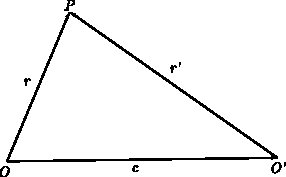
\includegraphics{figure/fig05.01}
    \caption{宇宙中的两个典型观察者$ O $及$ O' $}
    \label{fig:05.01}
\end{wrapfigure}
体质量密度为$  \rho \left( \vec{r} , t \right)   $。它的
意义是在$ t $时刻位于$ \vec{r} $的小
体积元$ \dif V $中的质量为
{\setlength\mathindent{3em}
\begin{equation*}
    \dif M = \rho \left( \vec{r} , t \right) \dif V
\end{equation*}}
类似地,$ O' $观察到的密度分
布写为$  \rho ' \left( \vec{r} ' , t \right)   $, $ \vec{r} ' $是相对于$ O' $的位置矢量。

由哥白尼原理,$ O $及$ O' $看到的密度分布应相同,即相对于$ O' $位
置矢量为$ \vec{r} ' $处的密度应等于相对于$ O $位置矢量为$ \vec{r} = \vec{r} ' $处的密度,
即
\begin{equation}\label{eqn:05.02.01}
    \rho ' \left( \vec{r} ' , t \right) = \rho \left( \vec{r} ' , t \right)
\end{equation}

另外,若分别由$ O $及$ O ' $观察同一点$ P $,其密度值当然应是一样
的,因为一个点只能有一个密度,故
\begin{equation}\label{eqn:05.02.02}
    \rho ' \left( \vec{r} ' , t \right) = \rho \left( \vec{r} , t \right)
\end{equation}
其中$ \vec{r} ' $及$ \vec{r} $之间满足下式
\begin{equation}\label{eqn:05.02.03}
    \vec{r} ' = \vec{r} - \vec{c}
\end{equation}
由式\eqref{eqn:05.02.01}、\eqref{eqn:05.02.02}、\eqref{eqn:05.02.03}可得
\begin{equation}\label{eqn:05.02.04}
    \rho \left( \vec{r} - \vec{c} , t \right) = \rho \left( \vec{r} , t \right)
\end{equation}
由于$ O $与$ O' $是可任意选的,即$ \vec{c} $取任何值上式都应成立。这样,
结论是\vspace{-1.2em}
\begin{equation}\label{eqn:05.02.05}
    \rho \left( 0 , t \right) = \rho \left( \vec{r} , t \right)
\end{equation}
这表示,物质的密度应与$ \vec{r} $无关,天体在大尺度上的分布应是均匀
的。这种密度分布一方面不与哥白尼原理矛盾,各个观察者都将
看到同样的均匀分布的天体;另一方面,它也能解释为什么可以
忽略无限多的星体在局部范围的引力效应,因为均匀分布是一种
对称分布。

现代天文观测的确已逐步证明,宇宙在大尺度的物质分布是
相当均匀的。